% Owner: Phat. ~1.5 pages.
\section{Results}\label{sec:results}

\begin{table}[t]
\centering
\caption{Exemplar-free CIL, ViT-B/16-IN21K. Top: reported by~\cite{rsiat} on the authors' partitions (one run).
Bottom: our runs, mean $\pm$ SD over 3 seeds; $\Delta$: paired difference to RSIAT with 95\% CI.
\TODOP{Rewrite the caption; decide how many published rows to keep (the ACL version has 10).
Springer discourages \texttt{\textbackslash resizebox} and \texttt{\textbackslash tiny}: consider moving the $\Delta$ rows to a separate small table.}}
\label{tab:main}
\resizebox{\textwidth}{!}{%
\begin{tabular}{lcccccccc}
\toprule
& \multicolumn{2}{c}{CIFAR-100} & \multicolumn{2}{c}{ImageNet-R} & \multicolumn{2}{c}{ImageNet-A} & \multicolumn{2}{c}{CUB-200} \\
\cmidrule(lr){2-3}\cmidrule(lr){4-5}\cmidrule(lr){6-7}\cmidrule(lr){8-9}
Method & $\bar A$ & $A_B$ & $\bar A$ & $A_B$ & $\bar A$ & $A_B$ & $\bar A$ & $A_B$ \\
\midrule
SLCA~\cite{zhang2023slca} & 94.09 & 91.53 & 81.17 & 77.00 & 68.66 & 58.74 & 89.51 & 82.19 \\
RanPAC~\cite{mcdonnell2023ranpac} & 94.35 & 90.86 & 82.98 & 77.94 & 69.32 & 61.82 & 93.13 & 89.40 \\
SSIAT~\cite{ssiat} & 94.35 & 91.35 & 83.63 & 79.38 & 70.83 & 62.43 & 93.38 & 89.53 \\
RSIAT~\cite{rsiat} & 95.15 & 92.20 & 86.92 & 82.75 & 74.89 & 66.23 & 93.99 & 90.59 \\
\midrule
RSIAT (ours) & 95.02{\tiny$\pm$.21} & 92.03{\tiny$\pm$.19} & 87.11{\tiny$\pm$.49} & 82.55{\tiny$\pm$.05}
 & 74.26{\tiny$\pm$1.1} & 67.02{\tiny$\pm$1.1} & 93.53{\tiny$\pm$.79} & 88.47{\tiny$\pm$.31} \\
SCF, ridge & 95.22{\tiny$\pm$.20} & 92.41{\tiny$\pm$.21} & 87.42{\tiny$\pm$.46} & 83.03{\tiny$\pm$.24}
 & 75.12{\tiny$\pm$1.2} & 67.69{\tiny$\pm$0.9} & 93.54{\tiny$\pm$.88} & 88.85{\tiny$\pm$.22} \\
SCF, PGM & 95.23{\tiny$\pm$.22} & 92.34{\tiny$\pm$.16} & 87.50{\tiny$\pm$.43} & 83.07{\tiny$\pm$.42}
 & 74.89{\tiny$\pm$1.0} & 67.65{\tiny$\pm$1.3} & 93.50{\tiny$\pm$.84} & 88.57{\tiny$\pm$.30} \\
\midrule
$\Delta$ ridge & $+$.20 {\tiny[.12,.28]} & $+$.38 {\tiny[.08,.69]} & $+$.32 {\tiny[.12,.51]} & $+$.48 {\tiny[.02,.94]}
 & $+$.85 {\tiny[.62,1.08]} & $+$.67 {\tiny[$-$.20,1.54]} & $+$.02 {\tiny[$-$.24,.27]} & $+$.38 {\tiny[.16,.61]} \\
$\Delta$ PGM & $+$.22 {\tiny[.15,.28]} & $+$.31 {\tiny[.18,.43]} & $+$.39 {\tiny[.25,.53]} & $+$.52 {\tiny[$-$.41,1.45]}
 & $+$.63 {\tiny[$-$.10,1.36]} & $+$.62 {\tiny[$-$.08,1.32]} & $-$.03 {\tiny[$-$.18,.12]} & $+$.10 {\tiny[.05,.16]} \\
\bottomrule
\end{tabular}}
\end{table}

\paragraph{SCF raises final accuracy on all four benchmarks.}
\TODOP{Read Table~\ref{tab:main} and Fig.~\ref{fig:gain}: A$_B$ rises by +0.38 to +0.67 (ridge), the CI excludes 0
on 3/4; $\bar A$ does not rise on CUB-200. Position against the published numbers, noting the different data splits.}

\begin{figure}[t]
\centering
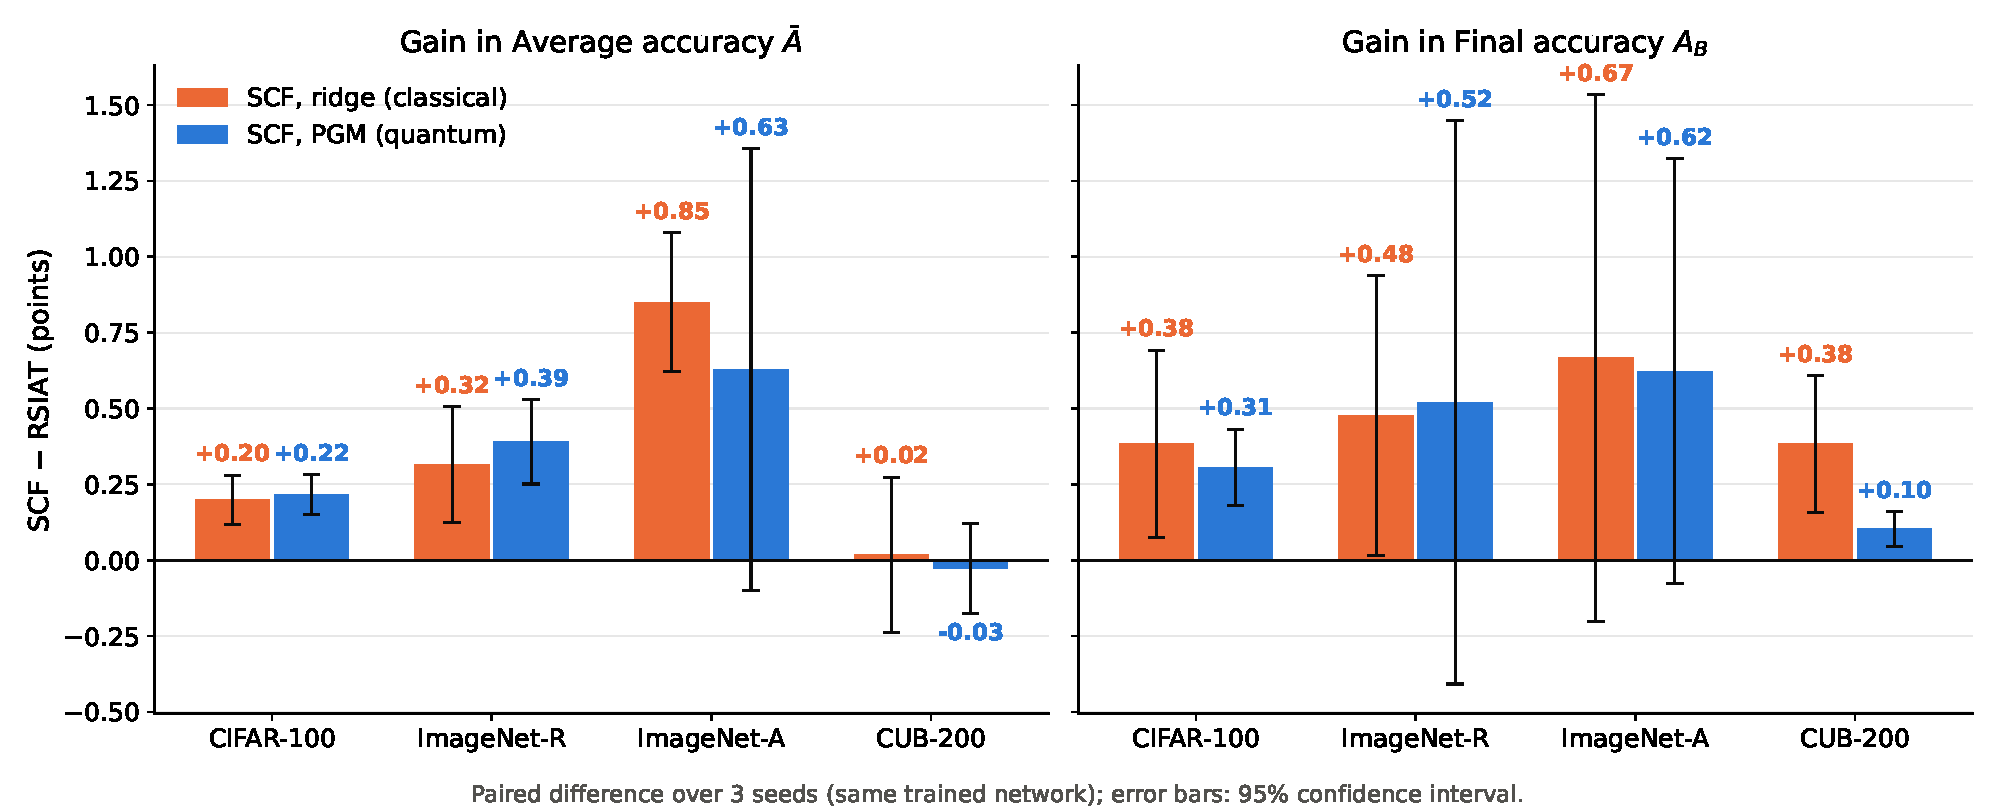
\includegraphics[width=\textwidth]{figures/scf_gain.pdf}
\caption{Paired gain of SCF over RSIAT (3 seeds, same network), 95\% CI. \TODOP{Rewrite the caption.}}
\label{fig:gain}
\end{figure}

\begin{table}[t]
\centering
\caption{Every quantum component against its classical twin (same inputs). $\Delta\bar A$ in points, paired
runs. R: ImageNet-R, A: ImageNet-A. \TODOP{Shorten/rewrite the caption; keep or drop the Holevo row.}}
\label{tab:twin}
\small
\begin{tabular}{lll r}
\toprule
Component & Comparison & $\Delta\bar A$ [95\% CI] & $n$ \\
\midrule
PQK, steering metric & PQK $-$ cosine, R & $+0.06$ [$-0.07$, $+0.18$] & 3 \\
PQK, separation (QKSR) & PQK $-$ RBF, R & $+0.07$ [$-0.01$, $+0.15$] & 3 \\
 & PQK $-$ no CNOT, R & $+0.04$ [$+0.04$, $+0.05$] & 3 \\
 & repaired $-$ original, R & $-0.07$ [$-0.11$, $-0.03$] & 3 \\
PQK, feature map & PQK ridge $-$ linear head, A & $-17.33$ [$-19.07$, $-15.59$] & 3 \\
Holevo objective & von Neumann $-$ MCR$^2$, R & $+0.06$ (screening) & 1 \\
PGM, stand-alone & PGM $-$ ridge, R+A & $+0.09$ [$-0.23$, $+0.40$] & 11 \\
PGM, fused (SCF) & PGM $-$ ridge, 4 datasets & $-0.04$ [$-0.17$, $+0.08$] & 12 \\
\bottomrule
\end{tabular}
\end{table}

\paragraph{The quantum score matches its classical twin.}
\TODOP{Read Table~\ref{tab:twin}: only one CI lies above 0 (+0.04); PGM = ridge, exactly as
Propositions~\ref{prop:unitary}--\ref{prop:scale} and the least-squares equivalence predict.}
